%%=============================================================================
%% Bevindingen
%%=============================================================================

\chapter{\IfLanguageName{dutch}{Bevindingen}{Findings}}%
\label{ch:bevindingen}

\section{Enkelvoudige requests}

De resultaten van de performantie testen voor de enkelvoudige requests met het REST API zonder compressie zijn terug te vinden in tabel ~\ref{tab:RESTenkelvoudigtabel}.
Elke lijn op deze tabel komt overeen met een uitgevoerde request. In de eerste kolom worden het aantal items die werden opgevraagd weergegeven,
in de tweede tot de vierde kolom de grootte van de dataset, in respectievelijk bytes, KB en MB, wanneer ze in JSON formaat naar een file worden weggeschreven,
daarna het tijdsverloop tussen de start van de request en het verkrijgen van de opgevraagde data in millie seconden. De zesde kolom geeft de de grootte van de
verzonden dataset per seconde dat de request geduurd heeft. Deze set van requests werd tweemaal uitgevoerd, in de laatste twee kolommen staat het resultaat, nl. het tijdsverloop en de snelheid,
van deze tweede set requests.
Op figuur ~\ref{fig:RESTenkelvoudigeRequestsFig} wordt de snelheid in MB/sec weergegeven ten opzichte van de grootte van de dataset. Hier werd tevens een trendlijn voorzien.

\begin{table}
    \centering
    \begin{tabular}{llllllll}
        \toprule
        \textbf{} & \textbf{} & \textbf{} & \textbf{} & \textbf{22/05/2023} & \textbf{} & \textbf{22/05/2023} & \textbf{} \\
        \midrule
        Items / call & Grootte set (bytes) & Grootte set (KB) & Grootte set (MB) & tijdsverloop (millies) & snelheid (Mb/s) & tijdsverloop (millies) & snelheid (Mb/s) \\
        1024 & 89028 & 86,94 & 0,08 & 67 & 1,194029851 & 69 & 1,15942029 \\
        2048 & 178062 & 173,89 & 0,17 & 131 & 1,297709924 & 130 & 1,307692308 \\
        4096 & 356103 & 347,76 & 0,34 & 223 & 1,524663677 & 261 & 1,302681992 \\
        8192 & 712225 & 695,53 & 0,68 & 429 & 1,585081585 & 445 & 1,528089888 \\
        9216 & 801209 & 782,43 & 0,76 & 470 & 1,617021277 & 473 & 1,606765328 \\
        10240 & 890124 & 869,26 & 0,85 & 525 & 1,619047619 & 533 & 1,594746717 \\
        11264 & 979136 & 956,19 & 0,93 & 608 & 1,529605263 & 587 & 1,584327087 \\
        12288 & 1068188 & 1043,15 & 1,02 & 627 & 1,626794258 & 629 & 1,621621622 \\
        13312 & 1157125 & 1130 & 1,1 & 689 & 1,596516691 & 681 & 1,615271659 \\
        14336 & 1246294 & 1217,08 & 1,19 & 789 & 1,508238276 & 752 & 1,582446809 \\
        15360 & 1335174 & 1303,88 & 1,27 & 784 & 1,619897959 & 784 & 1,619897959 \\
        16384 & 1424160 & 1390,78 & 1,36 & 832 & 1,634615385 & 836 & 1,626794258 \\
        20480 & 1780317 & 1738,59 & 1,7 & 1037 & 1,639344262 & 1057 & 1,608325449 \\
        24576 & 2136595 & 2086,52 & 2,04 & 1284 & 1,588785047 & 1297 & 1,572860447 \\
        28672 & 2492585 & 2434,17 & 2,38 & 1444 & 1,648199446 & 1723 & 1,381311666 \\
        32768 & 2848302 & 2781,54 & 2,72 & 1689 & 1,610420367 & 1673 & 1,625821877 \\
        36864 & 3204548 & 3129,44 & 3,06 & 1874 & 1,632870864 & 2465 & 1,24137931 \\
        40960 & 3560626 & 3477,17 & 3,4 & 2082 & 1,633045149 & 5177 & 0,656751014 \\
        45056 & 3916542 & 3824,75 & 3,74 & 2278 & 1,641791045 & 2278 & 1,641791045 \\
        49152 & 4272567 & 4172,43 & 4,07 & 2511 & 1,62086818 & 2612 & 1,558192956 \\
        53248 & 4628732 & 4520,25 & 4,41 & 2693 & 1,637578908 & 2737 & 1,611253197 \\
        57344 & 4984625 & 4867,8 & 4,75 & 3248 & 1,462438424 & 2888 & 1,644736842 \\
        61440 & 5341250 & 5216,06 & 5,09 & 3093 & 1,645651471 & 3128 & 1,627237852 \\
        65536 & 5697065 & 5563,54 & 5,43 & 3944 & 1,376774848 & 3351 & 1,620411817 \\
        131072 & 11394036 & 11126,99 & 10,87 & 8771 & 1,239311367 & 6707 & 1,620694796 \\
        262144 & 22788054 & 22253,96 & 21,73 & 13460 & 1,614413076 & 13412 & 1,620190874 \\
        524288 & 45575493 & 44507,32 & 43,46 & 28082 & 1,547610569 & 32374 & 1,342435288 \\
         &  &  &  &  &  &  &  \\
         &  &  & gemiddelde: &  & 1,551567585 &  & 1,50085742 \\
         &  &  & max: &  & 1,648199446 &  & 1,644736842 \\
         &  &  & min: &  & 1,194029851 &  & 0,656751014 \\
        \bottomrule
    \end{tabular}
    \caption{REST enkelvoudige requests}
    \label{tab:RESTenkelvoudigtabel}
\end{table}


\begin{figure}[ht]
    \centering
    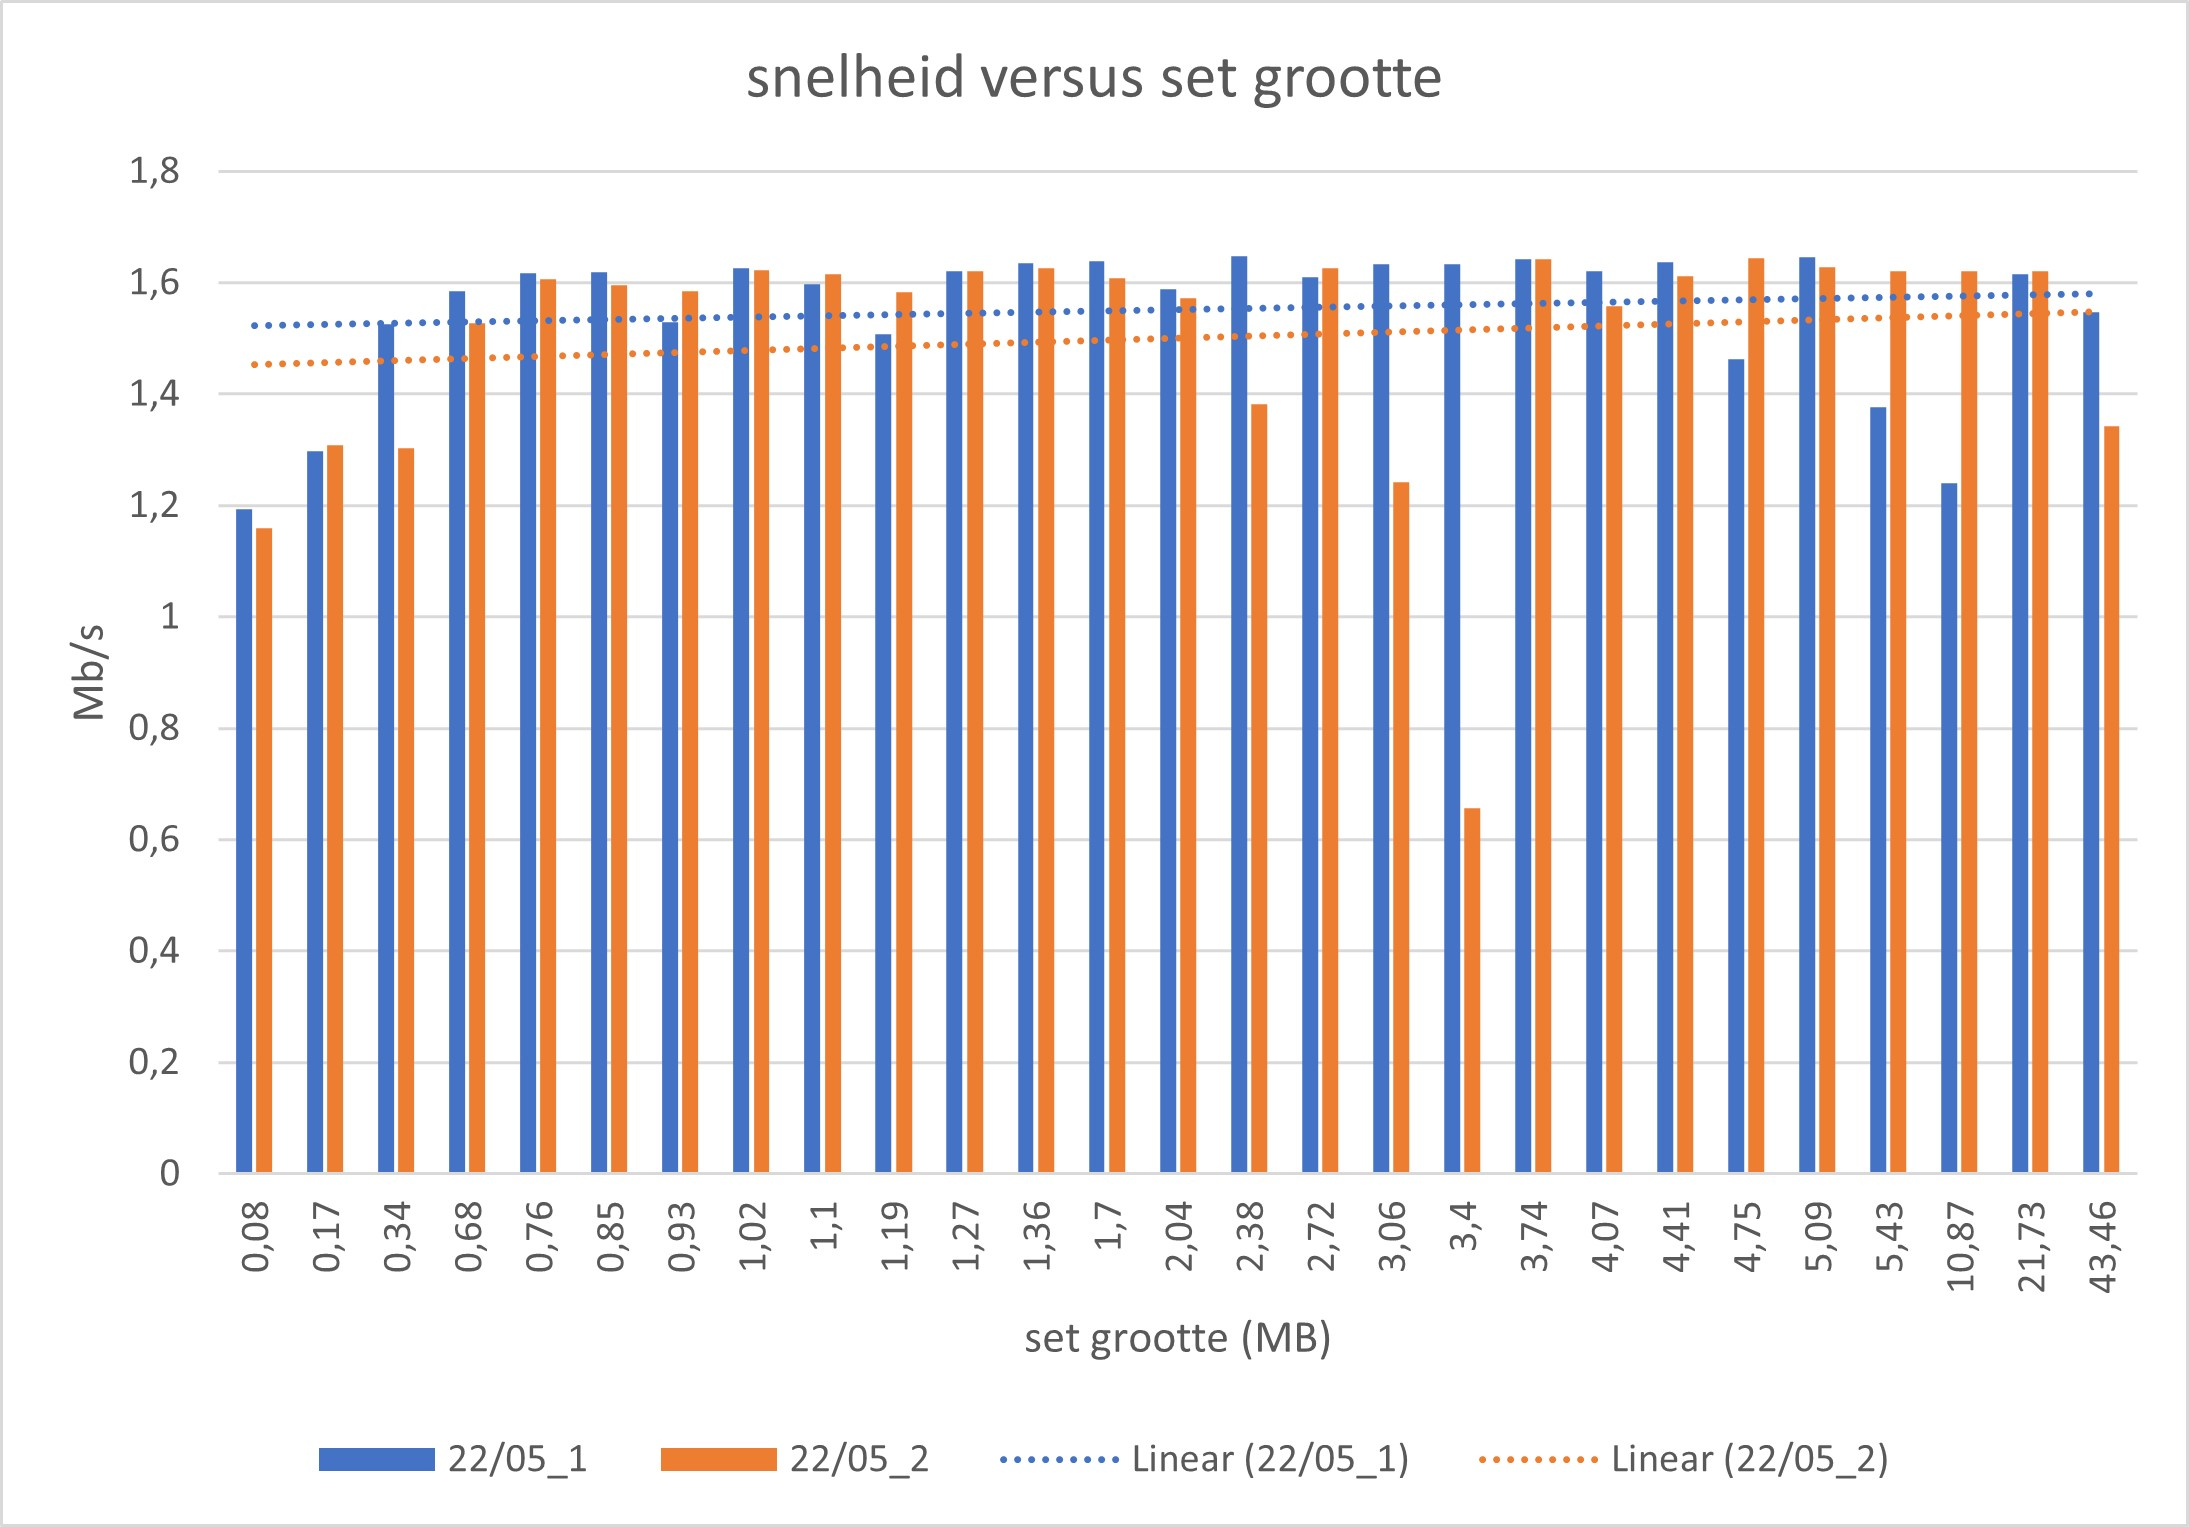
\includegraphics[width=1.0\linewidth]{RESTenkelvoudigeRequests}
    \caption{[REST enkelvoudige requests snelheid vs. grootte dataset]REST enkelvoudige requests snelheid vs. datasets van vari\"erende grootte}
    \label{fig:RESTenkelvoudigeRequestsFig}
\end{figure}

De resultaten van de performantie testen voor de enkelvoudige requests met de gRPC API functie getPeople, welke een object van het type Uni teruggeeft zijn
terug te vinden in tabel ~\ref{tab:gRPCUnienkelvoudigtabel}.
Op figuur ~\ref{fig:gRPCUnienkelvoudigeRequestsFig} wordt de snelheid \(MB/sec\) weergegeven ten opzichte van de grootte van de dataset. Hier werd tevens een trendlijn voorzien.


\begin{table}
    \centering
    \begin{tabular}{llllllll}
        \toprule
        \textbf{} & \textbf{} & \textbf{} & \textbf{} & \textbf{22/05/2023} & \textbf{} & \textbf{22/05/2023} & \textbf{} \\
        \midrule
        Items / call & Groote subset (bytes) & Groote subset (KB) & Groote subset (MB) & tijdsverloop (millies) & snelheid (Mb/s) & tijdsverloop (millies) & snelheid (Mb/s) \\
        1024 & 89028 & 86,94 & 0,08 & 48 & 1,666666667 & 66 & 1,212121212 \\
        2048 & 178062 & 173,89 & 0,17 & 64 & 2,65625 & 78 & 2,179487179 \\
        4096 & 356103 & 347,76 & 0,34 & 84 & 4,047619048 & 76 & 4,473684211 \\
        8192 & 712225 & 695,53 & 0,68 & 138 & 4,927536232 & 138 & 4,927536232 \\
        9216 & 801209 & 782,43 & 0,76 & 233 & 3,261802575 & 152 & 5 \\
        10240 & 890124 & 869,26 & 0,85 & 194 & 4,381443299 & 177 & 4,802259887 \\
        11264 & 979136 & 956,19 & 0,93 & 194 & 4,793814433 & 190 & 4,894736842 \\
        12288 & 1068188 & 1043,15 & 1,02 & 229 & 4,454148472 & 204 & 5 \\
        13312 & 1157125 & 1130 & 1,1 & 217 & 5,069124424 & 220 & 5 \\
        14336 & 1246294 & 1217,08 & 1,19 & 239 & 4,979079498 & 232 & 5,129310345 \\
        15360 & 1335174 & 1303,88 & 1,27 & 251 & 5,059760956 & 258 & 4,92248062 \\
        16384 & 1424160 & 1390,78 & 1,36 & 266 & 5,112781955 & 263 & 5,171102662 \\
        20480 & 1780317 & 1738,59 & 1,7 & 331 & 5,135951662 & 325 & 5,230769231 \\
        24576 & 2136595 & 2086,52 & 2,04 & 394 & 5,177664975 & 401 & 5,087281796 \\
        28672 & 2492585 & 2434,17 & 2,38 & 453 & 5,253863135 & 455 & 5,230769231 \\
        32768 & 2848302 & 2781,54 & 2,72 & 516 & 5,271317829 & 575 & 4,730434783 \\
        36864 & 3204548 & 3129,44 & 3,06 & 581 & 5,266781411 & 576 & 5,3125 \\
        40960 & 3560626 & 3477,17 & 3,4 & 649 & 5,238828968 & 639 & 5,320813772 \\
        45056 & 3916542 & 3824,75 & 3,74 & 707 & 5,289957567 & 695 & 5,381294964 \\
        49152 & 4272567 & 4172,43 & 4,07 & 766 & 5,313315927 & 794 & 5,125944584 \\
        53248 & 4628732 & 4520,25 & 4,41 & 826 & 5,338983051 & 819 & 5,384615385 \\
        57344 & 4984625 & 4867,8 & 4,75 & 895 & 5,30726257 & 909 & 5,225522552 \\
        61440 & 5341250 & 5216,06 & 5,09 & 1036 & 4,913127413 & 1612 & 3,157568238 \\
        65536 & 5697065 & 5563,54 & 5,43 & 1047 & 5,186246418 & 1266 & 4,289099526 \\
        131072 & 11394036 & 11126,99 & 10,87 & 2009 & 5,410652066 & 2030 & 5,354679803 \\
        262144 & 22788054 & 22253,96 & 21,73 & 4162 & 5,221047573 & 4080 & 5,325980392 \\
        524288 & 45575493 & 44507,32 & 43,46 & 8931 & 4,866196395 & 9030 & 4,812846069 \\
         &  &  &  &  &  &  &  \\
         &  &  &  & gemiddelde: & 4,763008315 &  & 4,728994056 \\
         &  &  &  & max: & 5,410652066 &  & 5,384615385 \\
         &  &  &  & min: & 1,666666667 &  & 1,212121212 \\
        \bottomrule
    \end{tabular}
    \caption{gRPC Uni enkelvoudige requests}
    \label{tab:gRPCUnienkelvoudigtabel}
\end{table}

\begin{figure}[ht]
    \centering
    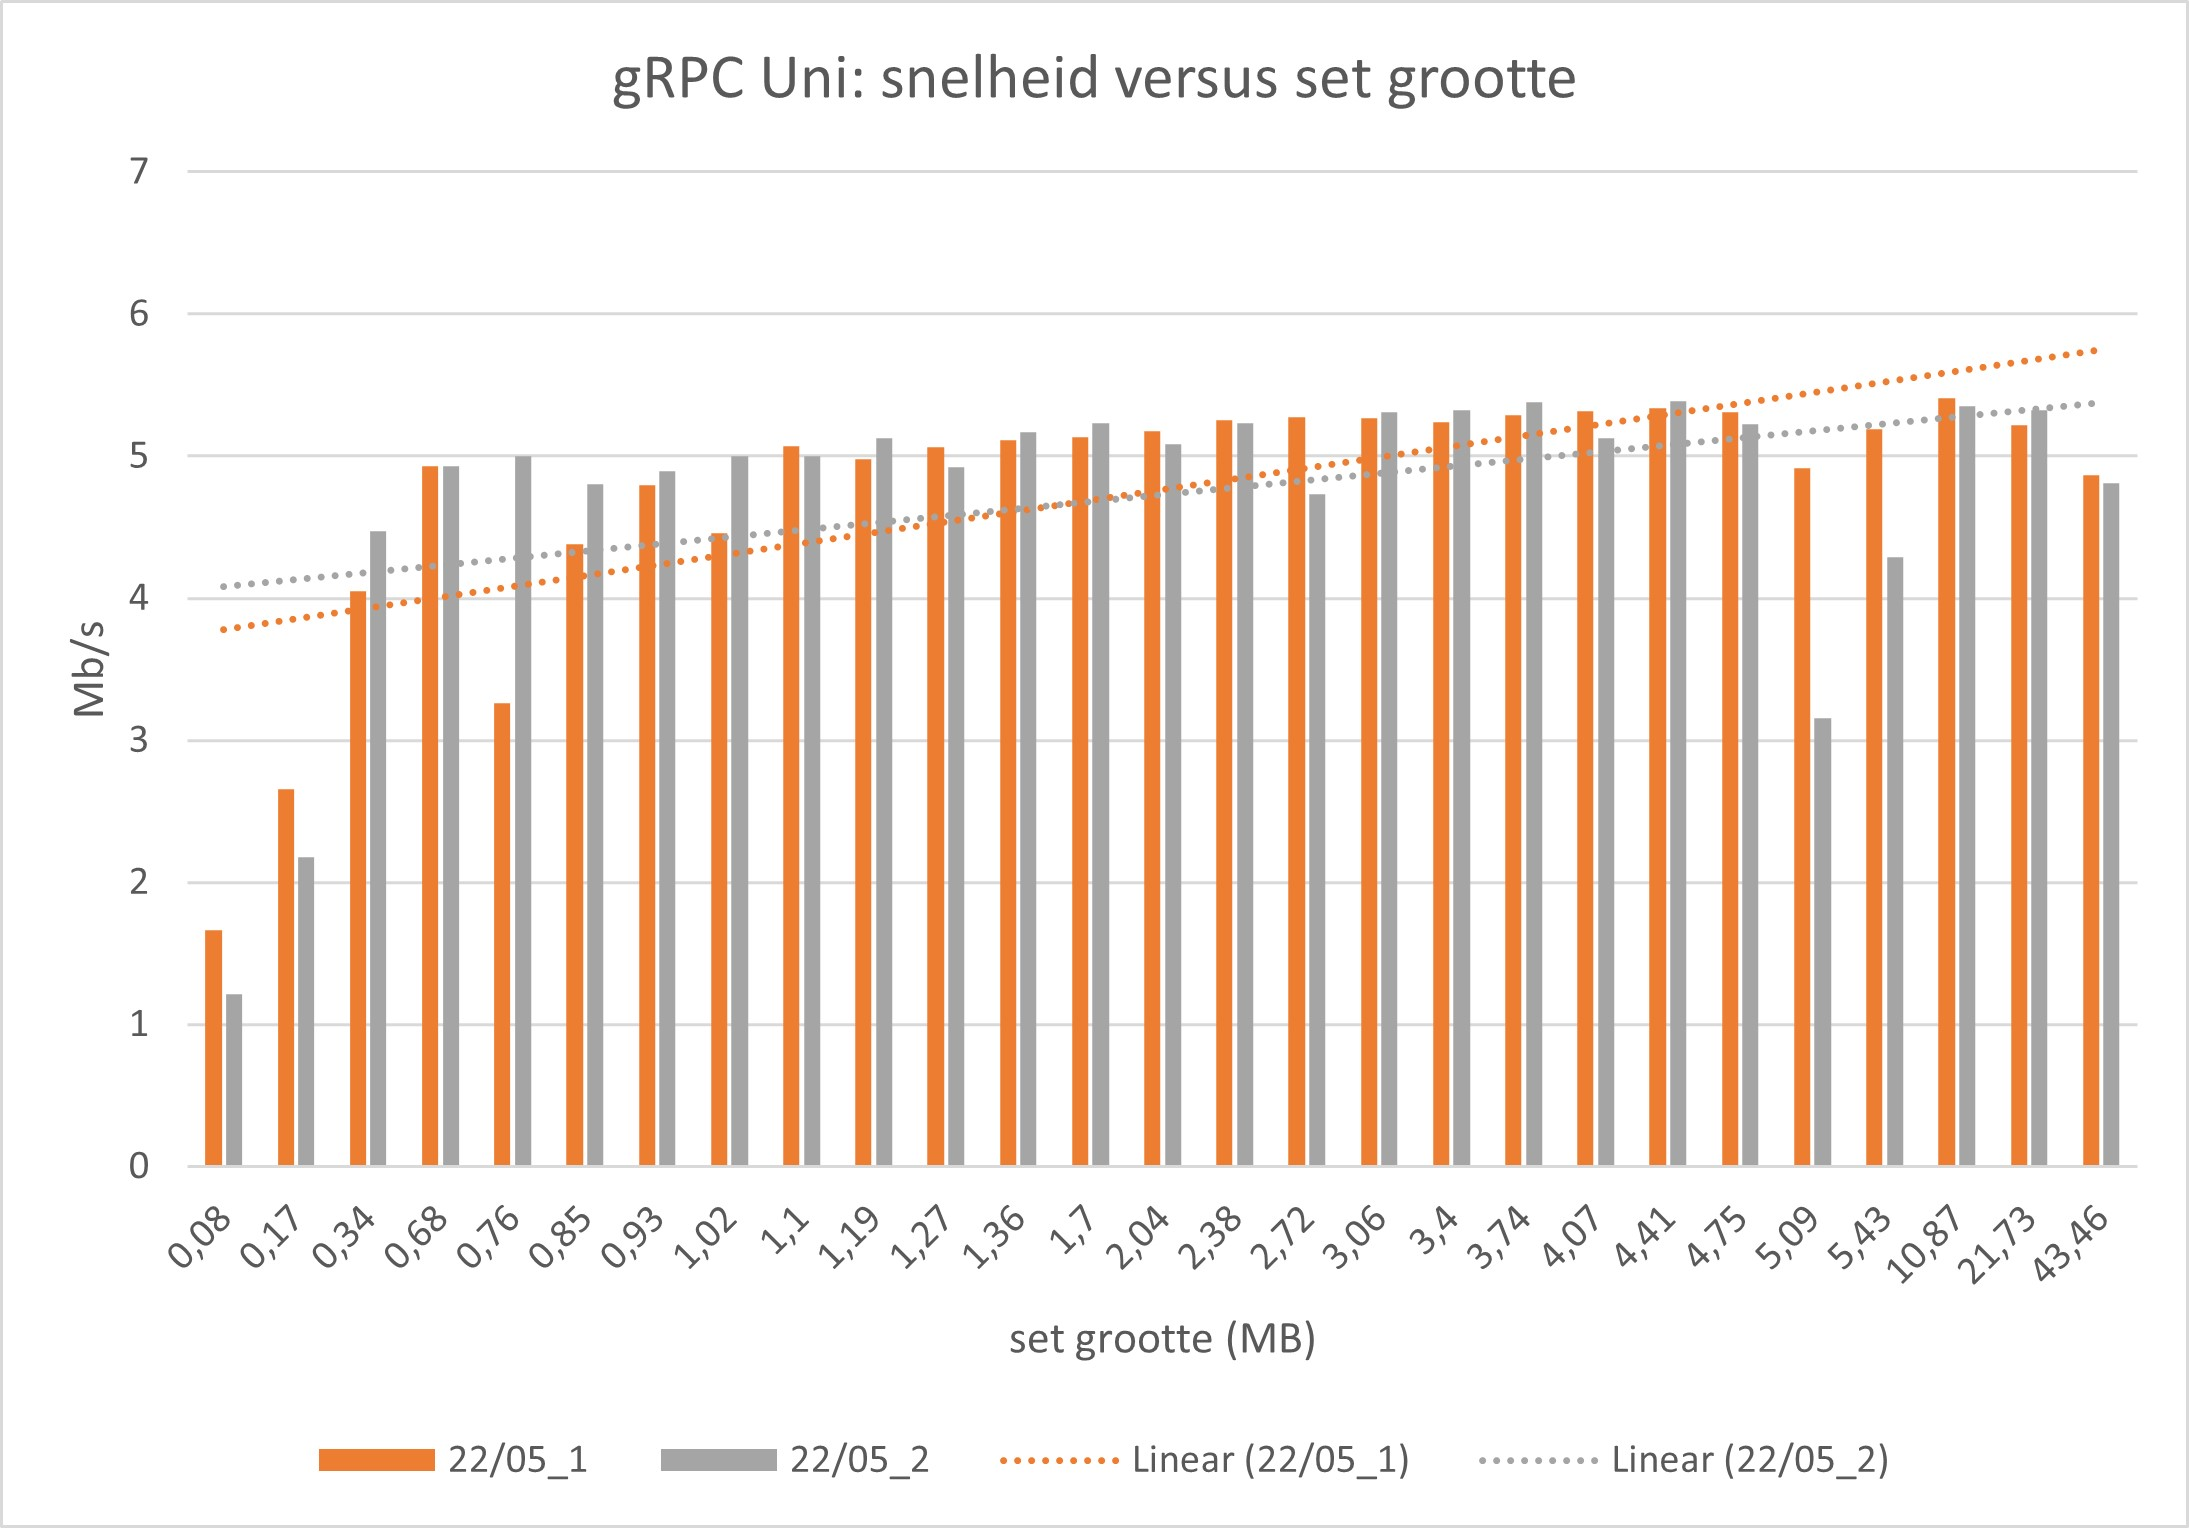
\includegraphics[width=1.0\linewidth]{gRPCUnienkelvoudigeRequests}
    \caption{[gRPC Uni enkelvoudige requests snelheid vs. grootte dataset]gRPC enkelvoudige requests snelheid vs. datasets van vari\"erende grootte}
    \label{fig:gRPCUnienkelvoudigeRequestsFig}
\end{figure}

De resultaten van de performantie testen voor de requests met de gRPC API functie getPeopleStream, welke een object van het type Multi teruggeeft zijn
terug te vinden in tabel ~\ref{tab:gRPCMultienkelvoudigtabel}.
Op figuur ~\ref{fig:gRPCMultienkelvoudigeRequestsFig} wordt de snelheid \(MB/sec\) weergegeven ten opzichte van de grootte van de dataset. Hier werd tevens een trendlijn voorzien.

\begin{table}
    \centering
    \begin{tabular}{llllll}
        \toprule
        \textbf{} & \textbf{} & \textbf{22/05/2023} & \textbf{} & \textbf{22/05/2023} & \textbf{} \\
        \midrule
        Groote subset (KB) & Groote subset (MB) & tijdsverloop (millies) & snelheid (Mb/s) & tijdsverloop (millies) & snelheid (Mb/s) \\
        86,94 & 0,08 & 41 & 1,951219512 & 45 & 1,777777778 \\
        173,89 & 0,17 & 52 & 3,269230769 & 68 & 2,5 \\
        347,76 & 0,34 & 88 & 3,863636364 & 89 & 3,820224719 \\
        695,53 & 0,68 & 164 & 4,146341463 & 163 & 4,171779141 \\
        782,43 & 0,76 & 180 & 4,222222222 & 184 & 4,130434783 \\
        869,26 & 0,85 & 231 & 3,67965368 & 214 & 3,971962617 \\
        956,19 & 0,93 & 216 & 4,305555556 & 219 & 4,246575342 \\
        1043,15 & 1,02 & 236 & 4,322033898 & 262 & 3,893129771 \\
        1130 & 1,1 & 252 & 4,365079365 & 259 & 4,247104247 \\
        1217,08 & 1,19 & 276 & 4,311594203 & 285 & 4,175438596 \\
        1303,88 & 1,27 & 293 & 4,33447099 & 295 & 4,305084746 \\
        1390,78 & 1,36 & 303 & 4,488448845 & 313 & 4,345047923 \\
        1738,59 & 1,7 & 374 & 4,545454545 & 399 & 4,260651629 \\
        2086,52 & 2,04 & 446 & 4,573991031 & 477 & 4,27672956 \\
        2434,17 & 2,38 & 526 & 4,524714829 & 538 & 4,423791822 \\
        2781,54 & 2,72 & 595 & 4,571428571 & 600 & 4,533333333 \\
        3129,44 & 3,06 & 658 & 4,650455927 & 674 & 4,540059347 \\
        3477,17 & 3,4 & 736 & 4,619565217 & 747 & 4,551539491 \\
        3824,75 & 3,74 & 802 & 4,663341646 & 846 & 4,420803783 \\
        4172,43 & 4,07 & 871 & 4,672789897 & 922 & 4,414316703 \\
        4520,25 & 4,41 & 954 & 4,622641509 & 966 & 4,565217391 \\
        4867,8 & 4,75 & 1011 & 4,698318497 & 1039 & 4,571703561 \\
        5216,06 & 5,09 & 1083 & 4,699907664 & 1131 & 4,500442087 \\
        5563,54 & 5,43 & 1177 & 4,613423959 & 1201 & 4,521232306 \\
        11126,99 & 10,87 & 2313 & 4,699524427 & 2358 & 4,609838846 \\
        22253,96 & 21,73 & 4616 & 4,707538995 & 4739 & 4,58535556 \\
        44507,32 & 43,46 & 9202 & 4,722886329 & 9291 & 4,677645033 \\
         &  &  &  &  &  \\
         & gemiddelde: &  & 4,327609997 &  & 4,186563708 \\
         & max: &  & 4,722886329 &  & 4,677645033 \\
         & min: &  & 1,951219512 &  & 1,777777778 \\
        \bottomrule
    \end{tabular}
    \caption{gRPC Multi}
    \label{tab:gRPCMultienkelvoudigtabel}
\end{table}

\begin{figure}[ht]
    \centering
    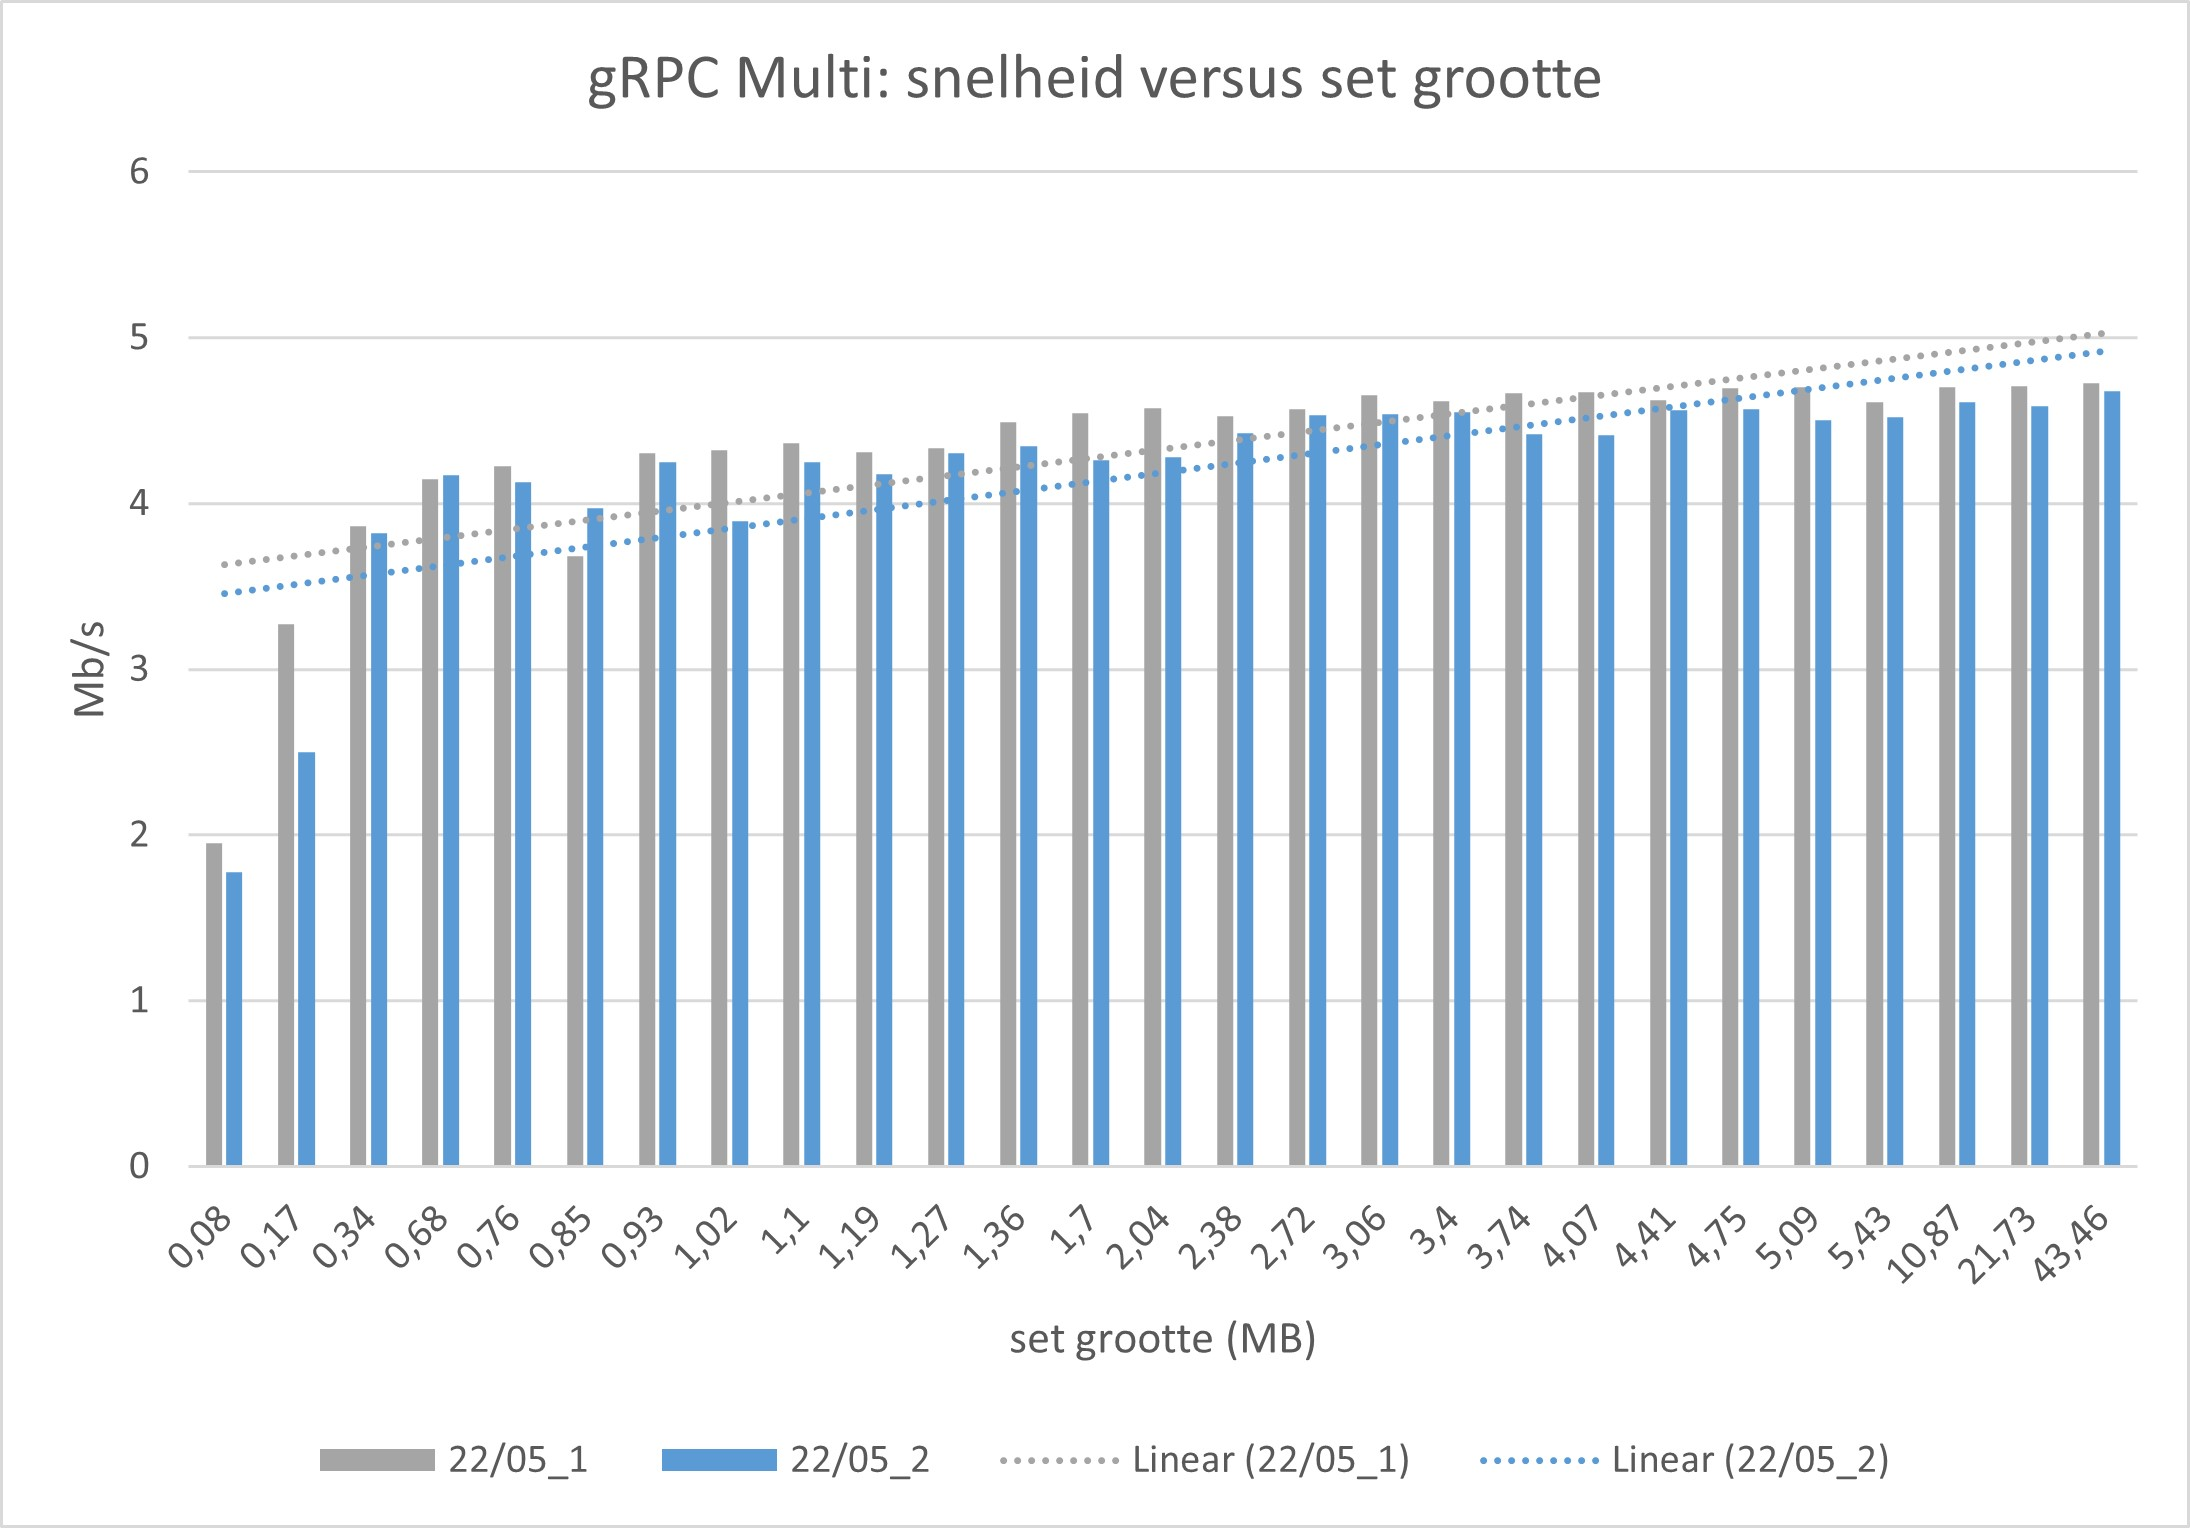
\includegraphics[width=1.0\linewidth]{gRPCMultienkelvoudigeRequests}
    \caption{[gRPC Multi snelheid vs. grootte dataset]gRPC Multi \(vgl. met enkelvoudige requests\) snelheid vs. datasets van vari\"erende grootte}
    \label{fig:gRPCMultienkelvoudigeRequestsFig}
\end{figure}

\section{Meervoudige requests}